\chapter{Overall Description}

\section{Product perspective}

\subsection{Scenarios}

\subsubsection*{Scenario 1: Automated Recording and Sensor-based Detection}
Daniele, an enthusiast cyclist, wants to track his daily commute to work. He opens the BBP app, logs in, and selects \emph{Start Cycling}. As he rides, the System automatically records his GPS Path. Suddenly, he hits a deep pothole; his smartphone vibrates violently. The System's algorithm analyses the accelerometer and gyroscope data and flags a potential obstacle at that location.

Upon reaching her destination, Daniele selects \emph{End Cycling}. The System presents a summary of the Trip, including performance statistics (speed, duration) and weather data (sunny, 22°C) retrieved from the external meteorological service. The System also asks him to validate the detected anomaly: \emph{We detected a strong vibration. Was this a pothole?}. Daniele confirms the detection. Finally, he decides to make this Path data public to warn other cyclists.

\subsubsection*{Scenario 2: Trip Planning with Data Merging and Freshness Analysis}
Stefano wants to plan a safe Sunday ride from his home to the city park. He navigates to the \emph{Discover} section and enters the source and destination points. The System calculates possible routes based on the available public data.

One direct route exists, but the System marks it with a low score and a \emph{Needs Maintenance} status. This happens because, although two Users rated it as \emph{Optimal} last month, three new Users reported \emph{Severe Potholes} yesterday. The System's merging algorithm prioritizes this fresher, confirming data. Consequently, BBP suggests an alternative, slightly longer route that has a high score and \emph{Optimal} status confirmed by recent Trips. Stefano chooses the safer alternative.

\subsubsection*{Scenario 3: Manual Path Creation and Management}
Matteo, an expert mountain biker, knows a shortcut through a forest trail that isn't mapped on standard road maps. He is currently at home and cannot ride it, so he logs into BBP and selects the \emph{Create a Path} section. 

Interacting with the map, he manually inputs the sequence of Segments connecting the entrance and exit of the trail. He assigns a specific status (\emph{Difficult}, \emph{Muddy}) to the route, which the System applies to all the involved Segments. Since he wants to immediately share this discovery with the community, he sets the visibility to \emph{Public} and confirms the creation. The System saves the Path and immediately updates the global map aggregation.

\subsubsection*{Scenario 4: Registration and Profile Setup}
Michele is a new User who wants to join the community. He downloads the app and selects \emph{Sign Up}. He provides his email, name, and password. After receiving an OTP code via email and verifying his identity, his account is active. He then accesses his profile to set his preferences. He is now ready to record Trips or browse the existing inventory of bike Paths.

\subsubsection*{Scenario 5: Guest Exploration (The Tourist)}
Tommaso is a tourist visiting the city for a weekend. He rents a bike and downloads BBP to find a safe route to the castle, but he does not want to create an account or share his personal details.

He selects \emph{Guest Login} (or \emph{Skip Registration}). The System allows him to access the \emph{Discover} section and search for Paths. He finds a highly-rated route and follows it using the map. However, when he tries to press \emph{Start Cycling} to record his performance, the System informs him that this feature requires a registered account. Tommaso declines the registration and continues to use the app solely for navigation and browsing public information.

\subsubsection*{Scenario 6: Smart Activity Detection and Trip Deletion}
Daniele starts a new recording for a training session. During the ride, he encounters a red traffic light and stops; the BBP System detects the zero speed and automatically pauses the recording to preserve the accuracy of the performance statistics. Later, he decides to get off the bike and walk it across a pedestrian area to grab a coffee. The System analyzes the accelerometer patterns and GPS speed, correctly identifying the activity as \emph{Walking} rather than \emph{Cycling}, and keeps the recording paused, ensuring the pedestrian Segment is not added to the bike Path inventory.

When Daniele resumes cycling, the System automatically wakes up and continues the tracking. At the end of the day, reviewing his \emph{My Trips} section, Daniele realizes this fragmented session is not useful for his long-term statistics. Since the System design ensures data integrity by disallowing manual modification of the recorded GPS track structure (to prevent data falsification), Daniele decides to discard the session entirely. He selects the Trip, taps \emph{Delete}, and confirms the action, permanently removing the data from the System.

\subsection{Domain Class Diagram}
The Domain Class Diagram (Figure \ref{fig:domain_class_diagram}) illustrates the conceptual model of the BBP System, defining the entities, their attributes, and the relationships that govern the System's logic. The model is designed to support the core requirements of crowdsourced data collection, Path reliability scoring, and User privacy.

\label{section:domain_class_diagram}
\begin{figure}[H]
    \centering
    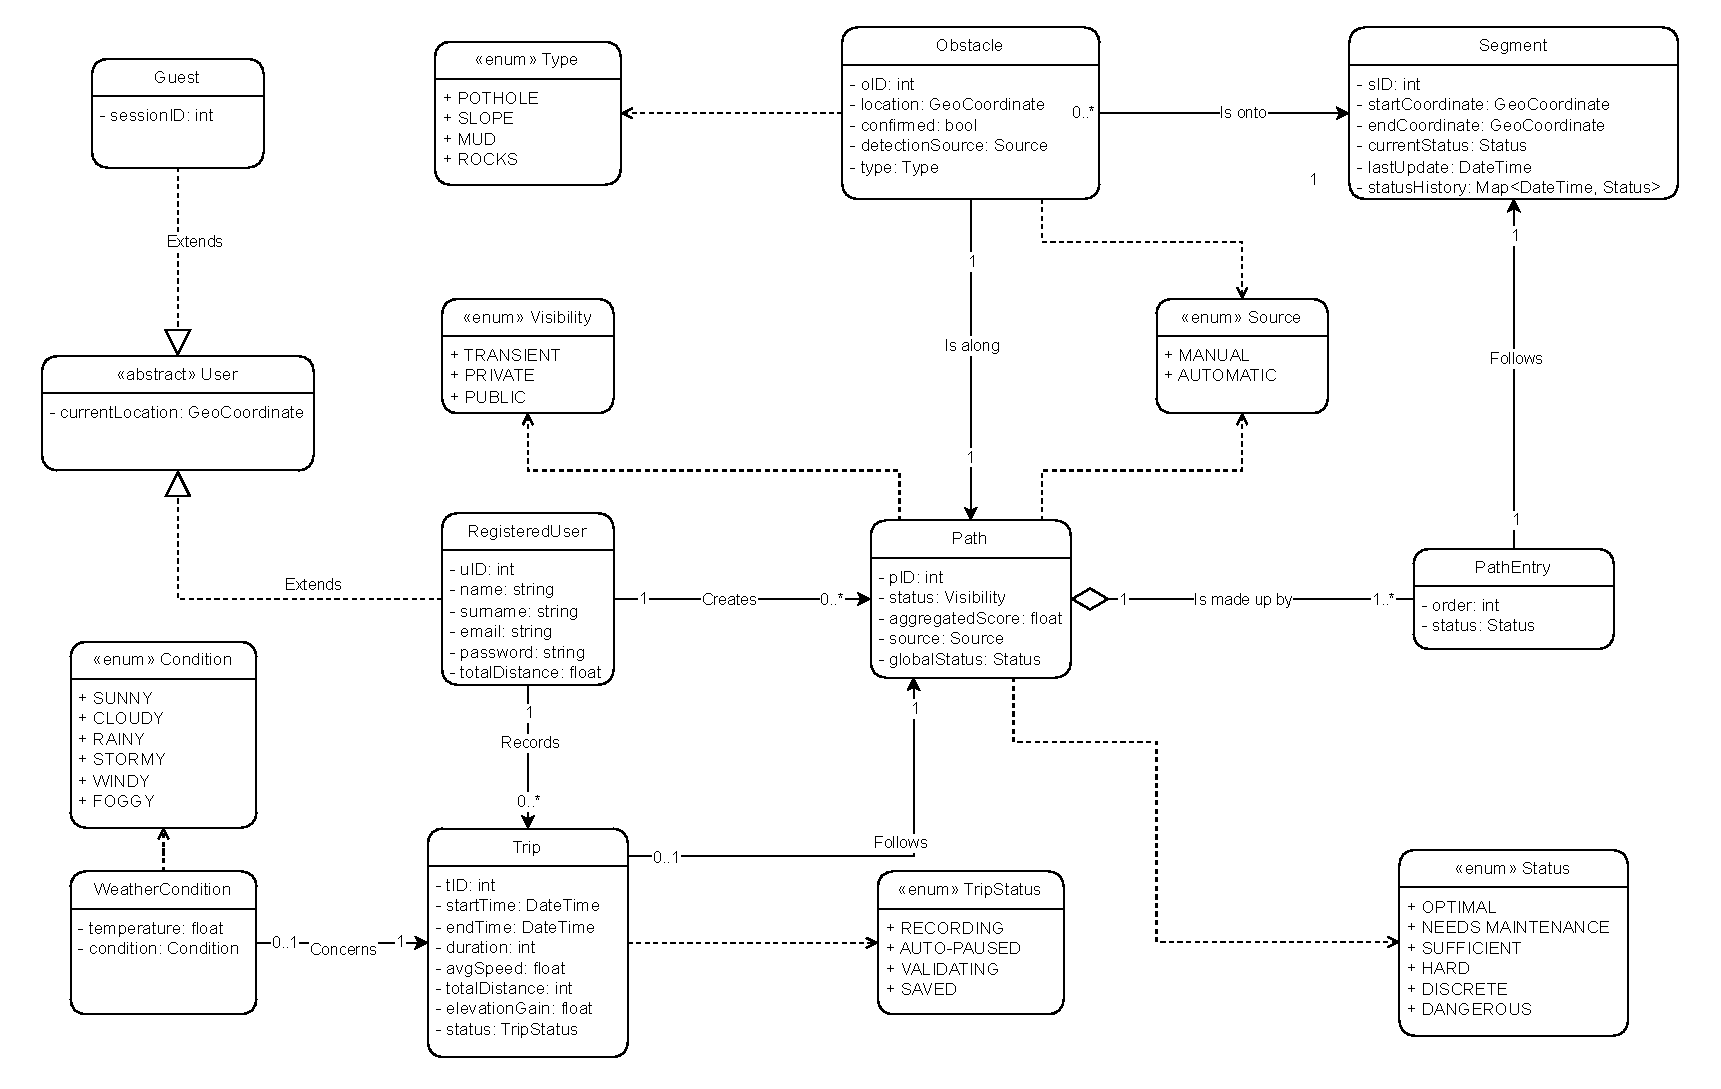
\includegraphics[width=0.99\textwidth]{pdf/domain_class_diagram.pdf}
    \caption{Domain Class Diagram for BBP}
    \label{fig:domain_class_diagram}
\end{figure}

The structure is centered around a clear separation between the \emph{Dynamic Activity} (the act of cycling) and the \emph{Static Geography} (the physical road network). This separation is crucial for the implementation of the Data Aggregation algorithm.

\subsubsection*{User Hierarchy}
The System defines a generalization hierarchy to manage different levels of access:
\begin{itemize}
    \item \textbf{User (Abstract)}: Represents the generalized concept of an actor interacting with the System via a mobile device. It holds the \texttt{currentLocation} (GeoCoordinate), which is the only attribute shared by all actors to enable map visualization and real-time tracking.
    \item \textbf{RegisteredUser}: Extends the generic User with persistent identity attributes (\texttt{email}, \texttt{password}), \texttt{name}, \texttt{surname}, and metrics such as \texttt{totalDistance}. This entity is the \emph{owner} of data: only a RegisteredUser can record \textbf{Trips} and create \textbf{Paths}.
    \item \textbf{Guest}: Represents an anonymous User. This entity has no persistent ID or profile data, consistent with the privacy-by-design approach, but inherits the capability to search and view the map. A \texttt{sessionID} is needed for session persistence.
\end{itemize}

\subsubsection*{Core Entities: Trip, Path, and Segment}
To satisfy the requirement of merging conflicting data from multiple Users while preserving the integrity of individual reports, the model adopts a normalized structure mediated by the \textbf{PathEntry} class:

\begin{itemize}
    \item \textbf{Trip}: 
    Represents the temporal event of a User cycling. It contains raw sensor data and performance metrics specific to that single session, such as \texttt{avgSpeed}, \texttt{totalDistance}, and \texttt{elevationGain}. 
    Crucially, it includes a \texttt{status} attribute (of type \texttt{TripStatus}) to track the recording lifecycle (\eg, Recording, Auto-Paused, Saved). A Trip is transient in nature; it documents \emph{what happened} at a specific time.
    
    \item \textbf{Path}: 
    Represents the immutable geographical definition of a route. It acts as a container for metadata such as \texttt{aggregatedScore} and \texttt{globalStatus}. 
    It holds a \texttt{status} attribute (of type \texttt{Visibility}) which manages the lifecycle and visibility of the route (\eg, Transient, Private, Public).
    The relationship between Trip and Path is defined as follows:
    \begin{itemize}
        \item A Trip \emph{follows} exactly one Path geometry (\texttt{1}).
        \item A Path is usually generated by a Trip, but can also be created manually without any recording. Hence, the multiplicity is \texttt{0..1} on the Trip side.
    \end{itemize}

    \item \textbf{PathEntry}: 
    This entity acts as the structural link between a user-defined Path and the physical road network. A Path is composed of a sequence of \texttt{PathEntries} (ordered by the \texttt{order} attribute).
    Crucially, \texttt{PathEntry} holds the \texttt{status} assigned by the user during that specific trip. This ensures that the user's subjective rating is encapsulated within their private Path data and is only propagated to the global map when the Path becomes Public.

    \item \textbf{Segment}: 
    This is the core entity for the \textbf{Data Aggregation} logic. A \texttt{Segment} represents a physical, atomic stretch of road (\eg, a specific street block or trail section) that exists independently of any User. 
    \begin{itemize}
        \item \textbf{Aggregation Logic}: The Segment holds the \texttt{currentStatus} (\eg, \emph{Muddy}) and the \texttt{lastUpdate} timestamp, representing the "global truth" visible to all users.
        \item \textbf{Status Propagation}: When a Path is published, the aggregation algorithm iterates through the list of \texttt{PathEntries}, taking the user-specific ratings and merging them into the \texttt{currentStatus} of the corresponding Segments. The Segment also maintains a \texttt{statusHistory} map to allow for data rollback and validation.
    \end{itemize}
\end{itemize}

\subsubsection*{Context and Anomalies}
The model includes entities to capture the environmental context of the ride:

\begin{itemize}
    \item \textbf{Obstacle}: Represents a hazard (\eg, \emph{Pothole}, \emph{Slope}) detected along a route. Obstacles lie on specific Segments and are connected to a specific Path.
    Crucially, the Obstacle includes a \texttt{detectionSource} attribute (defined in the \texttt{Source} enumeration) to distinguish between anomalies automatically detected by the sensors (accelerometer/gyroscope) and those manually inserted by the User during validation.
    
    \item \textbf{WeatherCondition}: Associated with every Trip, when available, it freezes the meteorological conditions (Temperature, Condition) at the time of the recording. This allows the System to filter statistics (\eg, \emph{Performance on rainy days}).
\end{itemize}

\subsubsection*{Enumerations}
To ensure data consistency, the model relies on strict enumerations for categorical data:
\begin{itemize}
    \item \textbf{Status}: Defines the quality of a Segment (Optimal, Sufficient, Hard, Dangerous).
    \item \textbf{Type}: Classifies the hazards (Pothole, Mud, Rocks).
    \item \textbf{Condition}: Standardizes weather reports (Sunny, Rainy, Foggy).
    \item \textbf{Source}: Distinguishes between Manual and Automatic obstacle detection.
    \item \textbf{TripStatus} and \textbf{Visibility}: Define the lifecycle states for the respective entities.
\end{itemize}
These enumerations can be extended with additional entries for a more detailed representation of different aspects of the object they refer to.
\subsection{State Diagrams}
To clarify the dynamic behaviour of the System's core entities, the following state diagrams illustrate the lifecycle of a \textbf{Trip} (focusing on the recording logic) and a \textbf{Path} (focusing on data persistence and visibility).


\subsubsection*{Trip Lifecycle}
Figure \ref{fig:Trip_state_diagram} models the User's recording session. It highlights the \emph{Smart Pausing} mechanism defined in requirement [R9], ensuring that stops or non-cycling activities do not pollute the performance statistics.

\begin{itemize}
    \item \textbf{Recording}: The active state where the System logs GPS coordinates and sensor data.
    \item \textbf{Auto-Paused}: Entered automatically when the System detects the speed has dropped below a threshold (for example, if the User is walking). In this state, data logging is suspended. The System automatically reverts to \emph{Recording} once cycling resumes.
    \item \textbf{Validating}: A transitional state entered upon pressing the \emph{Stop} button. Here, the data is frozen while the User confirms details about the Path and assigns a status (as per UC5). From here, the User can either confirm the session or discard it entirely.
    \item \textbf{Saved}: The final stable state where the Trip is persisted in the User's history (\emph{My Trips} section). It remains here until the User explicitly decides to delete it.
\end{itemize}

\subsubsection*{Path Lifecycle}
Figure \ref{fig:Path_state_diagram} illustrates the lifecycle of the geographical route definition, managing its visibility to the community. This logic is central to the \emph{Data Merging} requirements.

\begin{itemize}
    \item \textbf{Transient}: The Path is being defined (either by a recording session or manual drawing via UC7) but is not yet persisted in the database. If the creation is cancelled, the object is destroyed.
    \item \textbf{Private}: The Path is visible only to its creator and does not contribute to the global map statistics.
    \item \textbf{Public}: The User has explicitly shared the Path. In this state, the Path's Segment statuses are merged into the global heatmap using the aggregation algorithm. A Path can be toggled between \emph{Private} and \emph{Public} at any time, triggering a recalculation of the community data.
\end{itemize}


\begin{figure}[H]
    \begin{subfigure}{\textwidth}
        \centering
        \includegraphics[width=\textwidth]{pdf/Trip_state_diagram.pdf}
        \caption{State Diagram of a Trip}
        \label{fig:Trip_state_diagram}    
    \end{subfigure}
    \begin{subfigure}{\textwidth}
        \centering
        \includegraphics[width=\textwidth]{pdf/Path_state_diagram.pdf}
        \caption{State Diagram of a Path}
        \label{fig:Path_state_diagram}
    \end{subfigure}
    \caption{State Diagrams for Core Entities}
\end{figure}
\newpage
\section{Product functions}
The BBP Platform is designed to help cyclists manage their Trips and Paths flawlessly, with key features that help make the User experience friendly and optimal for monitoring and planning.

\begin{itemize}
    \item \textbf{User Access and Registration}: Users can sign up to the Platform to enable tracking features and contribute to the community data. The System also supports a \emph{Guest Mode}, allowing unregistered Users to browse the inventory and search for Paths without recording their activities.
    
    \item \textbf{Trip Tracking and Statistics}: The Platform provides a tracking functionality that Users can activate when starting a new Trip. While cycling, the application uses the built-in phone sensor System (GPS, accelerometer, gyroscope) to record the session and analyse performance (\eg, speed, duration). If available, the System enriches the Trip data with meteorological information retrieved from external services.
    
    \item \textbf{Automated Data Acquisition}: During a Trip, the System automatically detects the Path structure and identifies potential anomalies (\eg, potholes) by analysing sensor data. It features activity recognition to distinguish whether the User is cycling based on speed and movement patterns.
    
    \item \textbf{Data Validation}: To mitigate false positives in automated detection, the System provides an interface for Users to review, confirm, or correct the automatically detected obstacles and Path Segments before saving or publishing the Trip.
    
    \item \textbf{Manual Path Management}: The System allows Users to define Paths manually without cycling, by selecting Segments on a map and assigning a status (\eg, \emph{Optimal}, \emph{Needs Maintenance}) which applies to the selected road sections. Users can manage the visibility of their Paths, choosing to keep them private or share them with the community.
    
    \item \textbf{Data Aggregation and Reliability Analysis}: The System processes public information incoming from different Users to create a consolidated view of the bike Paths network. It merges conflicting reports by considering data freshness and the number of confirming sources to assign a reliability score and a unified status to each Path.
    
    \item \textbf{Smart Path Search}: Users can search for Paths between two locations. The System visualizes the results on a map, filtering and ranking the alternatives based on the calculated score, Path status, and overall efficiency.
\end{itemize}

\subsection{Requirements}

\subsubsection*{Account and Session}
\begin{rlist}
    % --- ACCOUNT & SESSION ---
    \item Upon request, the System shall allow a User to sign up to the Platform, as long as they provide all the required information and a profile is not already associated with it.
    \item Upon request, the System shall allow a User to log in to the Platform, as long as the correct credentials are provided.
    \item Upon request, the System shall allow a User to access the Platform as a guest.
    \item Upon request, the System shall allow a registered User to start a training session.
    \item Upon request, the System shall allow a registered User to end a training session, as long as they had already started it before.
\end{rlist}

\subsubsection*{Recording and Sensors}
\begin{rlist}[resume]
    % --- RECORDING & SENSORS ---
    \item Whenever a Trip is being recorded, the System shall keep track of the Path followed by the User acquiring GPS coordinates.
    \item Whenever a Trip is being recorded, the System shall analyze data from the device's accelerometer and gyroscope to automatically detect potential obstacles (\eg, potholes).
    \item Whenever the System detects a potential obstacle during a recording, it shall temporarily store its location and type for validation at the end of the session.
    \item Whenever a Trip is being recorded, the System shall automatically pause the data acquisition if the detected speed or movement pattern suggests the User is not cycling (\eg, walking or stationary).
\end{rlist}

\subsubsection*{Validation and Immutability}
\begin{rlist}[resume]
    % --- VALIDATION & IMMUTABILITY ---
    \item Upon concluding a recorded Trip (and before final storage), the System shall require the User to validate (confirm or delete) the automatically detected obstacles and assign a general status to the traversed Segments.
    \item Upon concluding a recorded Trip (and before final storage), the System shall allow the User to manually insert and classify obstacles that were not automatically detected by the sensors.
    \item The System shall prevent any modification to the Path's structural data (GPS track) and descriptive details (status, obstacles) once the Path has been saved to the System.
\end{rlist}

\subsubsection*{Manual Management}
\begin{rlist}[resume]
    % --- MANUAL MANAGEMENT ---
    \item Upon request, the System shall allow a registered User to insert a Path manually, as long as a list of streets and statuses is provided.
    \item Upon request, the System shall allow a registered User to delete their recorded Trips.
    \item Upon request, the System shall allow a registered User to delete their Paths, whether inserted manually or automatically.
\end{rlist}

\subsubsection*{Visibility}
\begin{rlist}[resume]
    % --- VISIBILITY ---
    \item Upon request, the System shall allow a registered User to make their Path available to the community (public), as long as said Path is currently private.
    \item Upon request, the System shall allow a registered User to make their Path private, as long as said Path has already been shared with the community.
    \item Upon request, the System shall allow a registered User to view all their Trips and Paths, whether they are private or public.
\end{rlist}

\subsubsection*{Data Merging and Algorithms}
\begin{rlist}[resume]
    % --- MERGING & ALGORITHMS ---
    \item Whenever a Path is made public, the System shall recalculate the status of the involved street Segments by aggregating the User's data with existing community data.
    \item When aggregating conflicting data about a Path Segment, the System shall prioritize information based on its freshness (recency of submission).
    \item When aggregating conflicting data about a Path Segment, the System shall resolve inconsistencies by considering the number of confirming reports from different Users.
    \item Whenever a public Path is made private or deleted, the System shall remove the specific User's contribution from the aggregated community data, triggering a recalculation of the Segment's status.
\end{rlist}

\subsubsection*{Statistics and Information}
\begin{rlist}[resume]
    % --- STATS & INFO ---
    \item Whenever a Trip is recorded, the System shall elaborate statistics on performance, such as estimated speed, total length, and time.
    \item Whenever a Trip is concluded and external weather services are available, the System shall retrieve and store the weather conditions associated with the Trip's location and time.
\end{rlist}

\subsubsection*{Search}
\begin{rlist}[resume]
    % --- SEARCH ---
    \item Upon request, the System shall provide a list of Paths connecting two locations to any User (registered or guest), visualizing them on a map ordered by their calculated score.
    \item Whenever providing search results, the System shall calculate a Path's score based on its aggregated status (\eg, optimal vs. bad) and its effectiveness in reaching the destination.
\end{rlist}

\section{User characteristics}
The BBP Platform is designed for two distinct categories of Users, differentiated by their level of interaction with the System's database:

\begin{table}[H]
    \sf
    \small
    \centering
    \renewcommand{\arraystretch}{1.5}
    \begin{tabularx}{\textwidth}{|l|X|}
        \hline
        \rowcolor{lightgray} \textbf{User} & \textbf{Characteristics} \\
        \hline
        \textbf{Registered Cyclists} &
        \textbf{Description}: Individuals who actively use the Platform not only to find routes but also to record Trips, monitor performance, and contribute data to the community.
        They span from \emph{proficient Users}, familiar with fitness apps and navigation technology, to \emph{novice Users} who may be less experienced with such interfaces.

        \textbf{Interaction Frequency}: Expert cyclists typically access the Platform multiple times per week for training. Recreational Users show seasonal variability (higher activity in spring/autumn and weekends).
        
        \textbf{Key Role}: They are the primary source of information for the System (crowdsourcing). Therefore, their ability to easily confirm or correct automated data is crucial for the System's reliability. \\
        \hline
        \textbf{Unregistered Users (Guests)} &
        \textbf{Description}: Individuals who wish to access the public inventory of bike Paths for exploration without account creation or performance tracking.

        \textbf{Interaction Frequency}: Highly unpredictable. This category includes tourists using the app for a single weekend or casual Users evaluating the service before registering.

        \textbf{Key Role}: They act solely as information consumers and cannot contribute new data or modify existing Paths. \\
        \hline
    \end{tabularx}
    \caption{User characteristics}
\end{table}

Given that the User base ranges from highly technical Users to complete beginners, and considering that data quality relies on User validation, the Platform must ensure a high usability standard. The interface must be straightforward enough for a casual User to navigate without training, yet comprehensive enough to provide detailed analytics for the expert cyclist.

\section{Assumptions, dependencies and constraints}
\subsection{Regulatory policies}
Since the BBP Platform collects and processes sensitive User data, specifically real-time geolocation (GPS) and movement patterns (via accelerometer and gyroscope), compliance with the \emph{General Data Protection Regulation (GDPR)} is mandatory.
Specific policies include:

\begin{itemize}
    \item \textbf{Data Anonymization}: Before being merged into the public knowledge base or used for statistical analysis, raw Trip data must be anonymized to prevent the identification of specific individuals or their private locations (\eg, home addresses).
    \item \textbf{Purpose Limitation}: Data is collected strictly for the purpose of service provision (Trip tracking, Path analysis) and must not be used for third-party commercial profiling or sold to advertisers.
    \item \textbf{Explicit Consent}: The System must obtain explicit User consent before accessing device sensors and location services.
\end{itemize}

\subsection{Domain Assumptions}
\label{domain_assumptions}
\begin{dalist}
    \item Users' GPS location is accurate.
    \item Users interact with the BBP application through a device with a functioning GPS connection. 
    \item Cyclists that decide to sign up have access to the mailbox of the provided email address.
    \item Users do not provide harmful information on Paths, such as suggesting cycling in dangerous areas or malicious routes.
    \item The majority of Users participate in the community with the intent of providing accurate information. Consequently, statistical aggregation of conflicting reports converges towards the actual state of the Paths.    
    \item Cyclists follow local traffic laws (\eg no access to highways, motorways, or forbidden/private streets).    
    \item Cyclists travel along physically defined tracks (roads, bike lanes, or beaten trails) and do not traverse open terrain where no Path exists (\eg, cutting diagonally across a field).
    \item The external map provider's database used by the System includes all physical Paths suitable for cycling, including off-road trails that might be missing from standard street navigation maps.
    \item During a Trip, cyclists rely only on their bicycle and do not switch to other means of transport (\eg cars, trains, buses) without stopping the recording.
    \item An Internet connection is available for data synchronization (Log In, Upload, Search), although it may be intermittent or absent during the cycling activity itself.
\end{dalist}